% Created 2020-07-21 mar 14:12
% Intended LaTeX compiler: pdflatex
\documentclass[presentation,aspectratio=1610]{beamer}
\usepackage[utf8]{inputenc}
\usepackage[T1]{fontenc}
\usepackage{graphicx}
\usepackage{grffile}
\usepackage{longtable}
\usepackage{wrapfig}
\usepackage{rotating}
\usepackage[normalem]{ulem}
\usepackage{amsmath}
\usepackage{textcomp}
\usepackage{amssymb}
\usepackage{capt-of}
\usepackage{hyperref}
\usepackage{khpreamble, euscript}
\DeclareMathOperator{\atantwo}{atan2}
\newcommand*{\ctrb}{\EuScript{C}}
\newcommand*{\obsv}{\EuScript{O}}
\usetheme{default}
\author{Kjartan Halvorsen}
\date{\today}
\title{Control computarizado - Retroalimentación de estados}
\hypersetup{
 pdfauthor={Kjartan Halvorsen},
 pdftitle={Control computarizado - Retroalimentación de estados},
 pdfkeywords={},
 pdfsubject={},
 pdfcreator={Emacs 26.3 (Org mode 9.3.6)}, 
 pdflang={English}}
\begin{document}

\maketitle

\section{Solución}
\label{sec:org119e12e}
\begin{frame}[label={sec:orgdc8d563}]{Solución del sistema en espacio de estados discreto}
El sistema
\begin{equation*}
x(k+1)=\Phi x(k) + \Gamma u(k), \quad x(0)= x_0
\end{equation*}
tiene la solución
\[x(n) = \Phi^n x_0 + \sum_{k=1}^n \Phi^{k-1} \Gamma u(n-k)\]

\alert{Verificación} Enseña \(x(n+1) = \Phi x(n) + \Gamma u(n)\)
\begin{align*}
x(n+1) &= \Phi^{n+1}x_0 + \sum_{k=1}^{n+1} \Phi^{k-1} \Gamma u(n+1-k)\\
       &= \Phi \Phi^{n}x_0 + \Phi \left( \sum_{k=2}^{n+1} \Phi^{k-2} \Gamma u(n+1-k) \right) + \Gamma u(n), \quad m = k-1\\
       &= \Phi \left( \Phi^{n}x_0 +  \sum_{m=1}^{n} \Phi^{m-1} \Gamma u(n-m) \right) + \Gamma u(n) 
       = \Phi x(n) + \Gamma u(n).
\end{align*}
\end{frame}


\begin{frame}[label={sec:orge172512}]{Solución del sistema discreto - ejercicio}
\begin{equation*}
x(k+1)=\Phi x(k) + \Gamma u(k), \quad x(0)= x_0
\end{equation*}
tiene la solución
\[x(n) = \Phi^n x_0 + \sum_{k=1}^n \Phi^{k-1} \Gamma u(n-k)\]

Calcula la respuesta al impulso del sistema 
\[ x(k+1) = \begin{bmatrix} 2 & 0\\0 & \frac{1}{2} \end{bmatrix} x(n) + \begin{bmatrix} 1\\1\end{bmatrix} u(k) \]

\begin{center}
  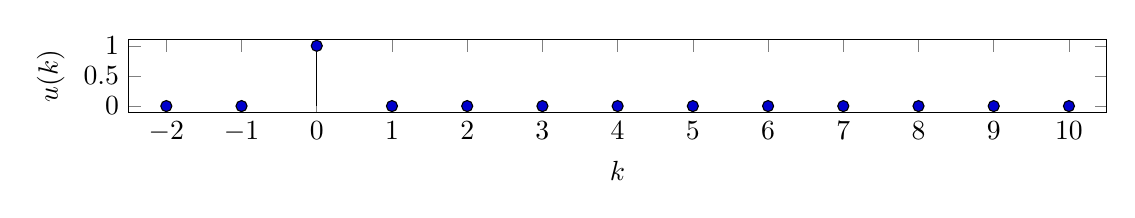
\begin{tikzpicture}
    \begin{axis}[
      width=14cm,
      height=2.5cm,
      xlabel={$k$},
      ylabel={$u(k)$},
      xmin=-2.5,
      xmax=10.5,
      ]

      \addplot+[black, ycomb, domain=-2:10, samples=13,variable=k] { (k==0) }; 

    \end{axis}
  \end{tikzpicture}
\end{center}
\end{frame}

\begin{frame}[label={sec:org73e3d60}]{Solución del sistema discreto - ejercicio}
\begin{equation*}
x(k+1)=\Phi x(k) + \Gamma u(k), \quad x(0)= x_0
\end{equation*}
tiene la solución
\[x(n) = \Phi^n x_0 + \sum_{k=1}^n \Phi^{k-1} \Gamma u(n-k)\]

Calcula la respuesta al impulso del sistema 
\[ x(k+1) = \begin{bmatrix} 2 & 0\\0 & \frac{1}{2} \end{bmatrix} x(n) + \begin{bmatrix} 1\\1\end{bmatrix} u(k) \]
Nota que \(x_0 = 0\) (sistema relajado), y que 
\[ \sum_{k=1}^n \Phi^{k-1} \Gamma u(n-k) = \Phi^{n-1}\Gamma = \begin{bmatrix}2 & 0\\0 & \frac{1}{2} \end{bmatrix}^{n-1} \begin{bmatrix}1\\1\end{bmatrix}\]
\end{frame}




\section{Estabilidad}
\label{sec:orgc1fdaf6}
\begin{frame}[label={sec:org85d792d}]{Estabilidad}
El sistema
\begin{equation*}
x(k+1)=\Phi x(k), \ \ x(0)=x_0
\end{equation*}
es \alert{estable} si  \(\underset{t\to\infty}{\lim}x(kh)=0, \quad \forall\;  x_0\in\Bbb{R}^n\).

Un requisito necessario y suficiente para estabilidad, es que \alert{todos los eigenvalores (valores característicos) de \(\Phi\) están en el interior del círculo unitario.}
\end{frame}

\begin{frame}[label={sec:org4f693fc}]{Eigenvalores y eigenvectores}
\alert{Definición} Eigenvalores \(\lambda\) y eigenvectores \(v\) de una matriz \(\Phi\) son pares \((\lambda, v \neq 0)\) que satisfican
\[ \Phi v = \lambda v \]
\end{frame}

\begin{frame}[label={sec:org05e9565}]{Eigenvalores y eigenvectores - ejercicio}
\alert{Actividad} Verifica que el vector 
\[ v = \begin{bmatrix}1\\0\end{bmatrix}\]
es un eigenvector de 
\[ \Phi = \begin{bmatrix} 2 & 0\\0 & \frac{1}{2} \end{bmatrix}. \]
Cuál es el eigenvalor correspondiente?
\end{frame}

\section{Controlabilidad y observabilidad}
\label{sec:org70f565f}

\begin{frame}[label={sec:org0ac3ca5}]{Controlabilidad}
Controlabilidad es la respuesta a la pregunta \emph{Podemos llegar a cualquier punto en el espacio de estados con una secuencia \(u(k),\; k=0,1,2,\ldots,n-1\) bien eligida?}

Considera
\[ x(k+1) = \Phi x(k) + \Gamma u(k), \quad x(0)= x_0 \]
con solución
\begin{equation}
\begin{split}
x(n) &= \Phi^nx(0) + \Phi^{n-1}\Gamma u(0) + \cdots + \Gamma u(n-1)\\
     &= \Phi^nx(0) + W_c U, 
\end{split}
\end{equation}
dónde
\begin{align*}
W_c &= \bbm \Gamma & \Phi\Gamma & \cdots & \Phi^{n-1}\Gamma\ebm\\
U &= \bbm u(n-1) & u(n-2) & \cdots & u(0) \ebm\transp
\end{align*}
\end{frame}

\begin{frame}[label={sec:orgd5d3d94}]{Reachability (controllability), contd}
To find the input sequence that takes the state to \(x(n) = x_d\) we solve the equation
\[ x_d = \Phi^nx(0) + W_cU\]
for \(U\). 

\[ U = W_c\inv \left(x_d - \Phi^nx(0)\right) \]

This requires the matrix \(W_x\) to be \alert{invertible}. This gives Theorem 3.7 in Å\&W:

THEOREM 3.7 REACHABILITY The state space system above is reachable if and only if the matrix \(W_c\) has rank \(n\). 

This is equivalent to 
\[ \det W_c \neq 0.\]
\end{frame}

\section{State feedback}
\label{sec:orge944b0d}
\begin{frame}[label={sec:orgc35dff8}]{State feedback}
Have state space model
 \begin{equation}
 \begin{split}
  x(k+1) &= \Phi x(k) + \Gamma u(k)\\
  y(k) &= C x(k)
 \end{split}
 \label{eq:ssmodel}
\end{equation}
and measurements (or estimates) of the state vector \(x(k)\). 

\alert{Linear state feedback} is the control law
\begin{equation*}
\begin{split}
 u(k) &= f\big((x(k), u_c(k)\big) = -l_1x_1(k) - l_2x_2(k) - \cdots - l_n x_n(k) + mu_c(k)\\
      &= -Lx(k) + mu_c(k), 
\end{split}
\end{equation*}
where \[ L = \bbm l_1 & l_2 & \cdots & l_n \ebm. \]

Insert the control law into the state space model \eqref{eq:ssmodel} to get
\end{frame}
\begin{frame}[label={sec:org1c644ea}]{State feedback}
Have state space model
 \begin{equation}
 \begin{split}
  x(k+1) &= \Phi x(k) + \Gamma u(k)\\
  y(k) &= C x(k)
 \end{split}
 \label{eq:ssmodel}
\end{equation}
and measurements (or estimates) of the state vector \(x(k)\). 

\alert{Linear state feedback} is the control law
\[ u(k) = -l_1x_1(k)  -l_2x_2(k) - \cdots - l_n x_n(k) + mu_c(k)= -Lx(k) + mu_c(k), \]
where \[ L = \bbm l_1 & l_2 & \cdots & l_n \ebm. \]

Insert the control law into the state space model \eqref{eq:ssmodel} to get
 \begin{equation}
 \begin{split}
  x(k+1) &= \left(\Phi -\Gamma L \right) x(k) + m\Gamma u_c(k)\\
  y(k) &= C x(k)
 \end{split}
 \label{eq:closedloop}
\end{equation}
\end{frame}

\begin{frame}[label={sec:org765bc1b}]{Pole placement by state feedback}
Assume the desired performance of the control system is given as a set of desired closed loop poles \(p_1, p_2, \ldots, p_n\), corresponding to the desired characteristic polynomial
\begin{equation}
a_c(z) = (z-p_1)(z-p_2)\cdots(z-p_n) = z^n + \alpha_1 z^{n-1} + \cdots \alpha_n.
\label{eq:desiredpoles}
\end{equation}

With state feedback we get the the closed-loop system
 \begin{equation}
 \begin{split}
  x(k+1) &= \left(\Phi -\Gamma L \right) x(k) + m\Gamma u_c(k)\\
  y(k) &= C x(k)
 \end{split}
 \label{eq:closedloop}
\end{equation}
with characteristic equation
\begin{equation}
\det\left(zI - (\Phi - \Gamma L)\right) = z^n + \beta_1(l_1,\ldots,l_n) z^{n-1} + \cdots \beta_n(l_1, \ldots, l_n).
\label{eq:poles}
\end{equation}

Equate the coefficients in \eqref{eq:desiredpoles} and \eqref{eq:poles} to get the system of equations
\begin{equation*}
\begin{split}
\beta_1(l_1, \ldots, l_n) &= \alpha_1\\
\beta_2(l_1, \ldots, l_n) &= \alpha_2\\
&\vdots\\
\beta_n(l_1, \ldots, l_n) &= \alpha_n
\end{split}
\label{eq:coeffs}
\end{equation*}
\end{frame}

\begin{frame}[label={sec:orgee03f04}]{Pole placement by state feedback, contd.}
The system of equations
\begin{equation*}
\begin{split}
\beta_1(l_1, \ldots, l_n) &= \alpha_1\\
\beta_2(l_1, \ldots, l_n) &= \alpha_2\\
&\vdots\\
\beta_n(l_1, \ldots, l_n) &= \alpha_n
\end{split}
\label{eq:coeffs}
\end{equation*}
is always linear in the unknown controller parameters, so it can be written
\begin{equation*}
A L\transp = \alpha,
\end{equation*}
Where \(\alpha\transp = \bbm \alpha_1 & \alpha_2 & \cdots & \alpha_n \ebm.\)
\end{frame}

\begin{frame}[label={sec:orgb2fe1da}]{Pole placement and reacability}
It can be shown that the controllability matrix \(W_c\) is a factor of the matrix \(A\)
\[ A = \bar{A} W_c. \] Hence, in general the system of equations
\begin{equation}
\bar{A}W_c L\transp = \alpha
\label{eq:poleplace}
\end{equation}
has a solution only if \(W_c\) is invertible, i.e. the system is \emph{reachable}.

Note that equation \eqref{eq:poleplace} can still have a solution for unreachable systems if \alert{\(\alpha\) is in the \emph{column space} of \(A\)}, i.e. \(\alpha\) can be written
\[ \alpha = b_1 A_{:,1} + b_2A_{:,2} + \cdots + b_mA_{:,m}, \; m < n \]
\end{frame}
\end{document}